\newpage
\section{Система компьютерной алгебры SageMath}
    \subsection{Обзор системы SageMath}
        SageMath~--- это свободная и открытая система компьютерной алгебры, 
        разработанная для решения широкого спектра математических задач. 
        Она объединяет в себе множество различных математических пакетов и 
        инструментов, обеспечивая пользователю возможность работы в единой среде.


        Цель создания системы SageMath заключалась в предоставлении математикам, 
        ученым и инженерам простого и эффективного способа решения математических 
        задач, без необходимости использования различных инструментов и пакетов. 
        Она позволяет проводить множество операций, начиная от простых 
        математических вычислений, заканчивая решением сложных дифференциальных 
        уравнений и построением трехмерных графиков.


        Одной из главных особенностей системы SageMath является её открытый и 
        расширяемый код, что позволяет пользователям модифицировать и дополнять 
        функциональность системы в соответствии с их потребностями. SageMath также 
        поддерживает различные языки программирования, такие как Python, Cython, 
        C, Fortran и др., что позволяет пользователям писать свои собственные 
        модули и расширения.
    \subsection{Особенности системы SageMath}
        SageMath предоставляет по сравнению с другими системами 
        компьютерной алгебры преимущества, в числе которых:
        \begin{enumerate}
            \item Бесплатность и открытый код~--- SageMath предоставляет 
            пользователю возможность использовать систему бесплатно и 
            иметь доступ к её исходному коду.
            \item Широкий спектр функциональности.
            \item Кроссплатформенность~--- SageMath может работать на 
            различных операционных системах, включая Windows, Mac OS и 
            многих дистрибутивах Linux.
            \item Простота в использовании~--- система предоставляет простой и 
            понятный интерфейс пользователя, что делает её использование 
            доступным даже для начинающих пользователей. Также, поскольку синтаксис в 
            SageMath идентичен синтаксису Python, освоение этой системы не требует 
            дополнительного изучения принципов написания программ в ней.
        \end{enumerate}
    \subsection{Работа с SageMath}
        Существует несколько вариантов работы в SageMath: терминал, веб-интерфейс SageMathCell и 
        Jupyter Notebook.


        Первый вариант похож на обычный интерпретатор Python, который удобно 
        использовать для небольших вычислений, поэтому для реализаций больших программ он 
        не подходит.


        Во втором варианте уже больше возможностей для написания большого количества кода. 
        Однако работа в SageMathCell требует подключения к интернету, а также не позволяет 
        разбивать код на несколько частей (ячеек), из-за чего при небольшом изменении в 
        программе приходится запускать все команды заново.


        Последний способ работы с SageMath исправляет многие недостатки предыдущих.
        Работа в формате ноутбука (.ipynb) позволяет разделять код на ячейки, выполянять их
        в любом порядке и при желании смотреть промежуточные результаты их выполнения.
\def\ord{\mathop{\mathrm{ord}}\nolimits}
\def\mat{\mathop{\mathrm{Mat}}\nolimits}
\def\rank{\mathop{\mathrm{rank}}\nolimits}
\def\lc{\ell c}
\def\max{\mathop{\mathrm{max}}\nolimits}

\newpage
\section{Матрицы дифференциальных операторов}
    \subsection{Основные понятия}
        Пусть $K$~--- дифференциальное поле характеристики 0 с производной
        $\partial =~'$. В дальнейшем будут использоваться следующие обозначения.
        Кольцо дифференциальных операторов с коэффициентами в $K$ обозначается через
        $K[\partial]$. Кольцо матриц размера $m \times m$ с элементами,
        принадлежащими кольцу $R$ обозначается через $\mat_m(R)$.


        Рассмотрим систему линейных дифференциальных уравнений $$L \cdot y(x)=0,$$
        где $L\in \mat_m(K[\partial])$, $y(x)$~---
        $m$--мерный вектор с компонентами $y_1(x),...,y_m(x)$.


        $L$ является матрицей дифференциальных операторов и может быть
        записана в виде $$L=A_r\partial^r+A_{r-1}\partial^{r-1}+\cdots+A_0,$$
        где $A_i \in \mat_m(K), i=0,...,r$. 


        Матрица $A_r$ ненулевая и
        называется \emph{ведущей} матрицей $L$. Число $r$ называется порядком $L$
        и обозначается как $\ord L$.


        Для обозначения $i$-й строки $L$ используется запись $L_{i,*}$.


        Строки $L_{1,*},...,L_{s,*} (s\leq m)$ называются независимыми над $K[\partial]$, если из того, что $f_1L_{1,*}+\cdots+f_sL_{s,*}=0$
        ($f_1,\ldots,f_s \in K[\partial]$) следует, что $f_1=\ldots=f_s=0$.
        \emph{Ранг} $L$~--- максимальное количество независимых строк.


        Пусть $\delta_i$~--- порядок строки $L_{i,*}$. Вектор
        $\delta=(\delta_1,...,\delta_m)$ называется вектором порядков строк~$L$.
        \emph{Фронтальной матрицей} называется такая матрица $L_0$, что $(L_0)_{i,*}=(A_{\delta_i})_{i,*}$.


        Матрица дифференциальных операторов $U \in \mat_m(K[\partial])$ называется \emph{унимодулярной} (или \emph{обратимой}), 
        если существует $U^{-1} \in \mat_m(K[\partial])$ такая, что $U^{-1}U=UU^{-1}=I_m$, где 
        $I_m$~---~единичная матрица размера $m\times m$.
        \subsection{Элементарные операции над строками}
        К элементарным операциям над строкам относятся следующие:
        \begin{enumerate}
            \item Перестановка двух строк.
            \item Умножение строки слева или справа на ненулевой элемент из $K$.
            \item Сложение строки с другой строкой, умноженной слева на 
            скалярный дифференциальный оператор из $K[\partial]$.
        \end{enumerate}


        Каждая элементарная операция по строкам соответствует умножению на элементарную 
        матрицу.
    \subsection{Приведение матрицы по строкам}
        Матрица $L$ называется \emph{приведённой по строкам}, если ненулевые строки
        её фронтальной матрицы независимы над $K[\partial]$. В случае, если $L$ полного ранга, 
        это означает обратимость фронтальной матрицы.


        Следующие три леммы показывают, что любая 
        матрица дифференциальных операторов может быть преобразована к 
        приведённому по строкам виду с помощью элементарных операций над строками:
        \begin{lemma}[\cite{frr}, \cite{rowred}]
            \label{lem:1}
            Пусть $L \in \mat_m(K[\partial])$ и $U,V \in \mat_m(K[\partial])$ 
            являются унимодулярными. Тогда ранги $L$, $UL$ и $LV$ равны.
        \end{lemma}
        \begin{lemma}[\cite{frr}, \cite{rowred}]
            \label{lem:2}
            Ранг приведённой по строкам матрицы дифференциальных операторов 
            равен рангу её фронтальной матрицы.
        \end{lemma}
        \begin{lemma}[\cite{frr}, \cite{rowred}]
            \label{lem:3}
            Пусть $L\in \mat_m(K[\partial])$ ранга $s \leq m$. Тогда всегда 
            можно построить унимодулярную матрицу $U\in \mat_m(K[\partial])$ 
            такую, что:
            $$UL=\left[
                \begin{array}{cc}
                    L^{*} \\ \hline
                    0
                \end{array}
            \right],$$
            где $L^{*}$~--- приведённая по строкам матрица дифференциальных операторов
            размера $s\times m$ такая, что $\ord~L^{*} \leq \ord~L$ и все её строки
            ненулевые.
        \end{lemma}
        Для полноты изложения приведём доказательство Леммы \ref{lem:3}.
        \begin{proof}
            Если $L$ уже приведена по строкам, то $U=I_m$, и дальнейшие вычисления
            проводить не нужно. Иначе, мы можем предположить, без потери общности, 
            что $L$ имеет все свои нулевые строки в нижней части матрицы. В таком 
            случае фронтальная матрица $L$ имеет вид:
            $$\left[
                \begin{array}{cc}
                    L_0 \\ \hline 0
                \end{array}
            \right],$$
            где $L_0$~--- фронтальная матрица первых $k$ строк $L$ ($k \geq s$). 
            Так как $L$ не приведена по строкам, то $L_0$ имеет ранг меньший $k$. 
            Тогда мы всегда можем найти ненулевой вектор $v=(v_1,\ldots ,v_k)$, 
            такой, что $vL_0=0$. Выберем индекс $t$, такой, что $v_t \neq 0$ и 
            $\delta_t=\max(\delta_i \neq 0)$. Определим $U_1 = 
            \mathrm{diag}(U_{11},I_{m-k})$, где
            $$U_{11}=\left[
                    \begin{array}{ccccccc}
                        1 & & & & & &\\
                        & \ddots & & & & &\\
                        & & 1 & & & &\\
                        v_1\partial^{\delta_t-\delta_1} & \cdots & v_{t-1}\partial^{\delta_t-\delta_{t-1}} & v_t & v_{t+1}\partial^{\delta_t-\delta_{t+1}} & \cdots & v_k\delta^{\delta_t-\delta_k}\\
                        & & & & 1 & &\\
                        & & & & & \ddots &\\
                        & & & & & & 1
                    \end{array}
                \right].$$


            Тогда $U_1$ является унимодулярной и при умножении на $L$ слева оставляет
            без изменений строки с индексами $i\neq t$ и заменяет $t$-ю строку на 
            $$\sum\limits_{i=1}^m v_i\partial^{\delta_t^{'}-\delta_i^{'}}L_{i,*}^{'}
                =\sum\limits_{i=1}^m v_i\lc(L_{i,*})\partial^{\delta_t}+p 
                =vL_0\partial^{\delta_t}+p=0+p=p,$$
            где $p$ обозначает элементы порядка, меньшего $\delta_t$.


            Таким образом, $t$-я строка $U_1L$ обладает порядком, меньшиим, чем $t$-я строка 
            $L$. Повторяя этот процесс конечное число раз, мы получим унимодулярную 
            матрицу дифференциальных операторов $U$, такую, что $UL$ будет иметь вид 
            $$UL=\left[
                    \begin{array}{cc}
                        L^{*} \\ \hline
                        0
                    \end{array}
                \right],$$
            где $L^{*}$~--- приведённая по строкам матрица дифференциальных операторов 
            размера $m_1 \times m$ ($m_1 \leq k$) с ненулевыми строками. Остаётся показать, что
            $m_1 = s$. Согласно лемме \ref{lem:1}, $\rank L=\rank UL
            =\rank L^{*}$. С одной стороны, согласно лемме \ref{lem:2}, ранг $L^{*}$ 
            равен рангу её фронтальной матрицы, то есть $m_1$. С другой стороны, $\rank L=s$, 
            поэтому $m_1=s$.
        \end{proof}
    \subsection{Алгоритм Row-Reduction}
        \label{r-r}
        Из доказательства леммы \ref{lem:3} следует алгоритм приведения матрицы по строкам, получивший название
        Row-Reduction.
        Дополнительно при этом строится унимодулярная матрица, которая пригодится
        далее для построения обратной матрицы.


        На вход алгоритма поступает матрица дифференциальных операторов $L\in \mat_m(K[\partial])$
        с порядком по строкам $\delta=(\delta_1,...,\delta_m)$ и порядком $\ord~L=l$.


        Далее необходимо инициализировать матрицу $L^{'}=L$ с порядком по строкам
        $\delta^{'}=(\delta_1^{'},...,\delta_m^{'})$, соответствующую ей фронтальную матрицу
        $L_0^{'}$ и матрицу $U=I_m$.


        Пока ненулевые строки $L_0^{'}$ зависимы над необходимо выполнять
        следующие шаги:
        \begin{enumerate}
            \item Вычислить ненулевой вектор $v=(v_1,...,v_m) \in K^{1\times m}$ такой, что $vL_0^{'}=0$.
            \item Выбрать целое число $t$ такое, что $v_t \neq 0, \delta_t^{'}=\max(\delta_i^{'},v_i\neq 0)$.
            \item Заменить $L_{t,*}^{'}$ на $\sum\limits_{i=1}^m v_i\partial^{\delta_t^{'}-\delta_i^{'}}L_{i,*}^{'}$.
            \item Заменить $U_{t,*}$ на $\sum\limits_{i=1}^m v_i\partial^{\delta_t^{'}-\delta_i^{'}}U_{i,*}$.
            \item Обновить $L_0^{'}$ и $\delta^{'}$.
        \end{enumerate}


        В результате на месте $L^{'}$ получается приведённая матрица дифференциальных операторов и
        унимодулярная матрица дифференциальных операторов $U$ такая, что $L^{'}=UL$.
    \subsection{Построение обратной матрицы}
        \label{rev}
        В статье \cite{abr_bark} приводится следующий факт, применимый к матрицам 
        дифференциальных операторов полного ранга:
        \begin{proposition}
            \label{prop1}
            Пусть $L\in \mat_m(K[\partial])$ имеет обратимую фронтальную матрицу. Тогда
            $L$ унимодулярна тогда и только тогда, когда $\ord~L=0$.
        \end{proposition}


        Алгоритм Row-Reduction, описанный в разделе~\ref{r-r}, позволяет вычислить унимодулярную матрицу $U\in \mat_m(K[\partial])$,
        такую, что $L^{'}=UL$ имеет обратимую фронтальную матрицу. Утверждение \ref{prop1}
        означает, что $L$ унимодулярна тогда и только тогда, когда $L^{'}$~--- обратиимая матрица в 
        $\mat_m(K)$. В таком случае $(L^{'})^{-1}UL=I_m$. Таким образом, 
        \begin{equation}
            \label{form}
            L^{-1}=(L^{'})^{-1}U.
        \end{equation}


\newpage
\section{Многочлены Оре}
    Теория колец многочленов Оре даёт возможность рассматривать различные 
    операторы, в частности линейные дифференциальные, с общей точки зрения. Это 
    позволяет создавать многоцелевые алгоритмы и соответствующие программы, 
    которые можно настраивать на конкретный вид операторов и уравнений. 


    Поэтому для представления операторных матриц в системе компьютерной алгебры SageMath 
    удобно использовать многочлены Оре.
    \subsection{Определение}
        Пусть $k$~--- поле характеристики 0, $\sigma: k \rightarrow k$~---
        автоморфизм $k$. Дифференцирование относительно $\sigma$~--- это любое отображение
        $\delta: k \rightarrow k$, для которого $\forall a,b \in k$
            $$\delta(a+b)=\delta a+\delta b$$
            $$\delta(ab)=\sigma(a)\delta b+\delta a b.$$


        \emph{Кольцо Оре} (или \emph{кольцо многочленов Оре}) над $k$, заданное посредством
        $\sigma$ и $\delta$ и обозначаемое $k[x;\sigma;\delta]$,~--- это кольцо
        многочленов от $x$ над $k$ с обычным сложением многочленов и умножением, 
        заданным формулой
            $$xa=\sigma(a)x+\delta a,~\forall a \in k.$$


        В~\cite{ore_abr} показано, что при $k=\mathbb{F}(t)$ (где $\mathbb{F}$~--- 
        любое подполе $\mathbb{C}$) в дифференциальном случае в качестве $\sigma$ 
        используется тождественное отображение на $k$, а в качестве $\delta$~--- 
        $\frac{d}{dt}$.
    \subsection{Поддержка в SageMath}
        Для работы с многочленами Оре в SageMath существует встроенный 
        функционал~(\cite{sage_ore}), который позволяет создавать кольца Оре над 
        коммутативными кольцами.


        К примеру, кольцо Оре дифференциальных операторов над $\mathbb{Q}[x]$ может 
        определяться следующим образом:
        \begin{lstlisting}[language=python]
            R.<x> = QQ[]
            der = R.derivation()
            A = OrePolynomialRing(R, der, 'D')
        \end{lstlisting}
        Иной способ определения:
        \begin{lstlisting}[language=python]
            A.<d> = R['D', der]
        \end{lstlisting}


        В результате создаётся следующий объект: \\
        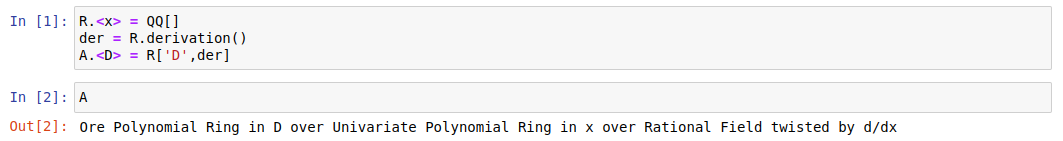
\includegraphics[width=\textwidth]{example1.png}


        Примеры вычисления произведения в описанном кольце Оре: \\
        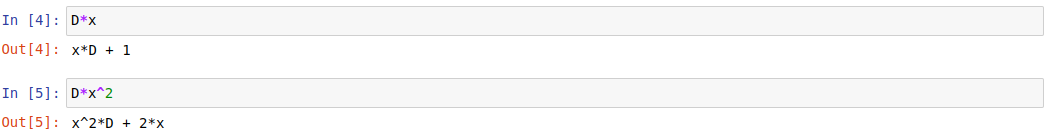
\includegraphics[width=\textwidth]{example2.png}

\newpage
\section{Реализация}
    \subsection{Описание алгоритма}
        Согласно выводам из раздела~\ref{rev}, можно сформулировать итоговый алгоритм 
        проверки унимодулярности матрицы дифференциальных операторов.
        \begin{enumerate}
            \item Преобразовать исходную матрицу к приведённому по строкам виду.
            \item Проверить, является ли полученная матрица обратимой в $\mat_m(\mathbb{Q}(x))$.
            \item Если является, то исходная матрица является унимодулярной, если нет, то не является.
        \end{enumerate}


        Далее, в случае положительного ответа, можно построить обратную матрицу для исходной 
        по формуле~\eqref{form}.

    \subsection{Примеры работы}
        Ниже рассмотерены примеры работы алгоритма.\\

        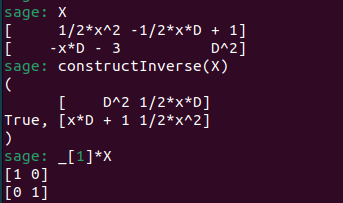
\includegraphics[width=0.75\textwidth]{im1.png}

        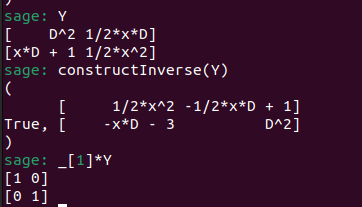
\includegraphics[width=0.75\textwidth]{im2.png}\\

        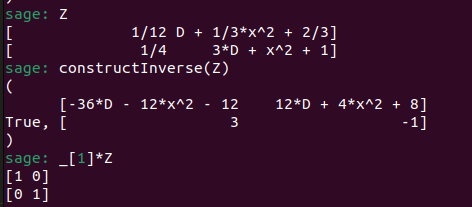
\includegraphics[width=0.75\textwidth]{im4.png}\\

        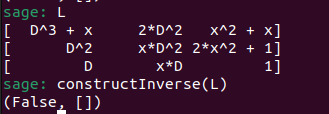
\includegraphics[width=0.75\textwidth]{im3.png}
\newpage
\section{Заключение}
    В ходе курсовой работы были получены следующие результаты:
    \begin{enumerate}
        \item Изучена система компьютерной алгебры SageMath.
        \item Изучен алгоритм Row-Reduction для приведения операторных матриц по строкам.
        \item Реализован алгоритм проверки унимодулярности матрицы 
        дифференциальных операторов и построения обратной матрицы 
        в системе компютерной алгебры SageMаth.
    \end{enumerate}


        Исходный код программы доступен по адресу: \url{https://github.com/MaxudMSU/unimodularity-course-work}.